%!TEX root = ../thesis.tex
%*******************************************************************************
%****************************** Second Chapter *********************************
%*******************************************************************************

\chapter{Caracterización Sucesos de Eventos}

\ifpdf
    \graphicspath{{Chapter2/Figs/Raster/}{Chapter2/Figs/PDF/}{Chapter2/Figs/}}
\else
    \graphicspath{{Chapter2/Figs/Vector/}{Chapter2/Figs/}}
\fi

Como se mencionó en el capitulo anterior, los sistemas WfM/BPM almacenan todos los sucesos de eventos generados al procesar cualquier elemento de trabajo. Estos sucesos de eventos, pueden estar relacionados por ejemplo con la creación de un nuevo elemento de trabajo, la asignación de un determinado elemento de trabajo a un usuario específico, la llegada de un elemento de trabajo a un cola específica, la invocación a un sistema externo, entre otras operaciones.

Específicamente para nuestro caso de estudio, los sucesos de eventos son almacenados en una única tabla, la cual se encuentran definida dentro de una base de datos relacional. La cantidad de registros de esta tabla crece con relación al número de elementos de trabajos procesados por el sistema, lo que quiere decir que para procesos que gestionan grandes cantidades de elementos de trabajo, se tienen grandes volúmenes de información. Esta tabla de sucesos de eventos cuenta con varios campos importantes, los cuales proveen información relevante al momento de intentar identificar el comportamiento de los elementos de trabajo.

En vista de lo anterior, y teniendo en cuenta que, el primer paso para abordar un problema haciendo uso de la inteligencia computacional es la caracterización de la base de datos, a continuación se describirá todo el proceso llevado a cabo para realizar dicha tarea.

%********************************** %First Section  **************************************
\section{Características de los Sucesos de Eventos} %Section - 2.1 
\label{section2.1}

Cada suceso de evento que es registrado por el sistema WfM tiene asociada cierta metadata. Esta metadata por un lado permite identificar cual fue el elemento de trabajo que generó dicha secuencia y el orden en que se generó, y por otro describe características importantes relacionadas con la generación del suceso de evento. Estas características se describen a continuación:

\begin{itemize}
    \item \textbf{Identificador del espacio de trabajo:} Esta característica permite identificar cual fue el espacio de trabajo usado por el elemento de trabajo que generó dicho suceso de evento. Es importante tener en cuenta, que un espacio de trabajo permite agrupar múltiples definiciones de flujos de trabajo.
    
    \item \textbf{Identificador de operación:} Esta característica almacena el identificador de la operación que se ejecutó en el elemento de trabajo que generó determinado suceso de evento. Estas operaciones se definen en los flujos de trabajo, y pueden corresponder por ejemplo a crear un documento en el contenedor de documentos, invocar un servicio web externo, ejecutar una funcionalidad específica, entre otras.
    
    \item \textbf{Identificador de la clase de trabajo:} Los sistema WfM cuentan con diferentes clases de trabajo, esta característica almacena el identificador interno de la clase de trabajo a la que pertenece el elemento de trabajo que generó el suceso de evento.
    
    \item \textbf{Identificador de la clase ejecutante:} Esta característica almacena el identificador interno de la clase que ejecuta el trabajo de la cola que contiene el elemento de trabajo en mención.
    
    \item \textbf{Tipo de evento:} Esta característica corresponde al identificador del evento que generó dicho sucesos de evento. Existen múltiples eventos que se pueden presentar al ejecutar los elementos de trabajo dentro del sistema WfM. En la tabla \ref{table:tipos_eventos} se describen algunos ejemplos de estos eventos, y las categorías a las que están asociados. 
    
    \item \textbf{Originador del elemento de trabajo:} Generalmente los elementos de trabajo son iniciados por un usuario, esta característica almacena el identificador del usuario que inició dicho flujo.
    
    \item \textbf{Asunto del elemento de trabajo:} Al definir los flujos de trabajo desde las herramientas de diseño, es posible asignarles un determinado asunto, esto con el fin de identificar a que proceso o subproceso corresponde. Por lo tanto esta característica almacena dicha información.
    
    \item \textbf{Respuesta de despacho:} Como se mencionó en la sección \ref{section1.2}, los elementos de trabajo son presentados a los usuarios finales por medio de in-baskets. Dentro de estos in-baskets, los usuarios pueden "avanzar" los elementos de trabajo a lo largo del proceso asociándoles algún tipo de respuesta. La anterior información es la que se encuentra almacena en dicha característica.
    
\end{itemize}

\begin{table}
    \centering
    \begin{tabular}{l | p{10cm}}
        \toprule
            \textbf{Categorías de eventos} & \textbf{Ejemplos de eventos presentados} \\
        \toprule
            \multirow{4}{*}{Instrucción de Traza} 
                & \multicolumn{1}{p{10cm}}{Cuando determinado elemento de trabajo finaliza, esta es una operación del sistema.} \\
                \cmidrule{2-2}
                & Cuando el nombre del elemento de trabajo es modificado. \\ 
        \midrule
            \multirow{2}{*}{Creación} 
                & \multicolumn{1}{p{10cm}}{Cuando se crea un elemento de trabajo hijo.} \\
                \cmidrule{2-2}
                & Cuando se crea un elemento de trabajo padre. \\ 
        \midrule
            \multirow{2}{*}{Terminación} 
                & \multicolumn{1}{p{10cm}}{Cuando se finaliza un elemento de trabajo hijo.} \\
                \cmidrule{2-2}
                & Cuando se finaliza un elemento de trabajo padre. \\ 
        \midrule
            \multirow{2}{*}{Mensaje de Administración} 
                & \multicolumn{1}{p{10cm}}{Cuando un elemento de trabajo es forzado a terminar.} \\
                \cmidrule{2-2}
                & Cuando un elemento de trabajo se elimina forzadamente. \\ 
        \midrule
            \multirow{3}{*}{Comienzo de operación} 
                & \multicolumn{1}{p{10cm}}{Cuando el procesador de pasos, o un usuario bloquea el elemento de trabajo.} \\
                \cmidrule{2-2}
                & Cuando un elemento de trabajo es encolado. \\ 
        \midrule
            \multirow{12}{*}{Fin de operación} 
                & \multicolumn{1}{p{10cm}}{Cuando un elemento de trabajo es actualizado y despachado para la siguiente cola.} \\
                \cmidrule{2-2}
                & Cuando un elemento de trabajo que se esta procesando finaliza de manera anormal. \\ 
                \cmidrule{2-2}
                & Cuando un elemento de trabajo es actualizado y desbloqueado en la misma cola. \\ 
                \cmidrule{2-2}
                & Cuando un elemento de trabajo es delegado a otro usuario. \\ 
                \cmidrule{2-2}
                & Cuando un elemento de trabajo es reasignado a otro usuario. \\ 
                \cmidrule{2-2}
                & Cuando un elemento de trabajo es finalizado y la operación del usuario es abortada. \\ 
        \midrule
            \multirow{2}{*}{Pasos del sistema} 
                & \multicolumn{1}{p{10cm}}{Cuando un paso es ejecutado sin especificarse una cola.} \\
                \cmidrule{2-2}
                & Cuando un paso compuesto es completado. \\ 
        
        \bottomrule
    \end{tabular}
    \caption[Ejemplo de eventos presentados en una herramienta WfM/BPM]{Algunas de las categorías que agrupan los diferentes eventos que se pueden presentar en una herramienta WfM/BPM, también da algunos ejemplos de dichos eventos. Es importante tener en cuenta que cada herramienta WfM/BPM define sus propios eventos, al igual que les asigna identificadores únicos.}
    \label{table:tipos_eventos}
\end{table}

Existen otras características que no se tuvieron en cuenta para este estudio, pues no se consideran relevantes para el proceso que se lleva acabo en este investigación. 


%********************************** %Second Section  **************************************
\section{One Hot Encoding} %Section - 2.2 
\label{section2.2}

Todas las características de los sucesos de eventos que se mencionaron en la sección anterior son variables categóricas, esto quiere decir que los valores de cada característica pueden ser fijos, o contar con un número limitado de elementos. Por ejemplo, la característica que permite identificar la clase de trabajo de cualquier elemento de trabajo, solamente contiene seis valores diferentes. Sin embargo, características como el identificador del usuario, o la respuesta de despacho pueden cambiar en el tiempo. Este último aspecto, implica que se debe tener sumo cuidado al momento de modelar los datos.

De acuerdo a lo anterior, y teniendo en cuenta que los modelos de machine learning no presentan buenos resultados al momento de trabajar con variables categóricas, es necesario realizar un proceso de conversión sobre dichas variables. Uno de los métodos más populares para realizar esta transformación es el llamado One Hot Encoding.

La técnica de One Hot Encoding sugiere la creación de nuevas columnas sobre la base de datos, donde cada nueva columna corresponde al valor de alguna de las categorías de las características existentes. Además, el valor de esta nueva columna será uno si determinado registro se encuentra asociado a dicha categoría, y cero en caso contrarío. La tabla \ref{table:ejemplo_categorias} muestra como podría visualizarse la información original de cada suceso de evento. Por otro lado, en la tabla \ref{table:ejemplo_onhotencoding} se muestra la nueva estructura de los datos luego de realizar el proceso de transformación usando One Hot Encoding, como se puede ver en esta tabla el resultado es un nuevo conjunto de vector binario para cada suceso de evento.

Después de realizar la categorización de los sucesos de eventos, y habiendo obtenido los vectores binarios correspondientes. Es una buena idea convertir dichos vectores binarios a su valor entero, dado que es más fácil su manipulación y almacenamiento. Lo anterior se puede visualizar en la figura \ref{table:ejemplo_onhotencoding} en la última columna. 

\begin{table}
    \centering
    \begin{tabular}{||c || c || c || c||} 
        \hline
            Workflow Id & Originator Id & Event Type & Operation Id \\ [0.5ex] 
        \hline\hline
            208aefee-e047 & 1 & 1 & 3 \\ 
        \hline
            208aefee-e047 & 2 & 2 & 1 \\
        \hline
            208aefee-e047 & 4 & 3 & 2 \\
        \hline
            208aefee-e047 & 2 & 4 & 4 \\
        \hline
            208aefee-e047 & 3 & 5 & 3 \\
        \hline
            208aefee-e047 & 1 & 6 & 2 \\
        \hline
    \end{tabular}
    \caption[Ejemplo características sucesos de eventos]{Algunos datos de ejemplo donde se puede ver como están estructuradas algunas de las características de los sucesos de eventos.}
    \label{table:ejemplo_categorias}
\end{table}

\begin{table}
    \centering
    \begin{tabular}{|| c || c | c | c | c || c | c | c | c | c | c || c | c | c | c || c ||} 
        \hline
            \multirow{2}{*}{Workflow Id} 
            & \multicolumn{4}{c ||}{Originator Id} 
            & \multicolumn{6}{c ||}{Event Type} 
            & \multicolumn{4}{c ||}{Operation Id} 
            & \multirow{2}{*}{Integer} \\ 
        \cmidrule{2-15}
            & 1 & 2 & 3 & 4 & 1 & 2 & 3 & 4 & 5 & 6 & 1 & 2 & 3 & 4 & \\ 
        \hline\hline
            208aefee-e047 & 1 & 0 & 0 & 0 & 1 & 0 & 0 & 0 & 0 & 0 & 0 & 0 & 1 & 0 & 8706 \\
        \hline
            208aefee-e047 & 0 & 1 & 0 & 0 & 0 & 1 & 0 & 0 & 0 & 0 & 1 & 0 & 0 & 0 & 4360 \\
        \hline
            208aefee-e047 & 0 & 0 & 0 & 1 & 0 & 0 & 1 & 0 & 0 & 0 & 0 & 1 & 0 & 0 & 1156 \\
        \hline
            208aefee-e047 & 0 & 1 & 0 & 0 & 0 & 0 & 0 & 1 & 0 & 0 & 0 & 0 & 0 & 1 & 4161 \\
        \hline
            208aefee-e047 & 0 & 0 & 1 & 0 & 0 & 0 & 0 & 0 & 1 & 0 & 0 & 0 & 1 & 0 & 2082 \\
        \hline
            208aefee-e047 & 1 & 0 & 0 & 0 & 0 & 0 & 0 & 0 & 0 & 1 & 0 & 1 & 0 & 0 & 8212 \\
        \hline
    \end{tabular}
    \caption[Ejemplo resultados luego de aplicar One Hot Encoding]{Resultado luego de realizar la transformación de One Hot Encoding sobre los datos de ejemplo mostrados en la tabla \ref{table:ejemplo_categorias}.}
    \label{table:ejemplo_onhotencoding}
\end{table}


%********************************** %Third Section  **************************************
\section{Métodos de cuantización vectorial} %Section - 2.3 
\label{section2.3}

Los datos obtenidos luego de realizar el proceso de One Hot Encoding presentan una particularidad, pues los valores obtenidos en la última columna de la tabla \ref{table:ejemplo_onhotencoding} no representan una secuencia continua, condición requerida para hacer uso de los modelos de inteligencia computacional propuestos en este trabajo. Por otro lado, los diferentes valores en esta columna pueden contener información duplicada, lo que representa un gran numero de elementos a analizar, y que podría afectar el desempeño de los modelos de inteligencia computacional que se pretenden usar.

A partir de lo anterior, surge la necesidad de usar lo que se denominan métodos de cuantización vectorial. El objetivo de la cuantización vectorial es mapear los vectores de secuencias desde un espacio de datos dado, a un conjunto finito de vectores de secuencias representados de manera sencilla, reduciendo de manera significativa el esfuerzo requerido para su almacenamiento y manipulación, al igual que eliminando información redundante \cite{Fink2014}. Dicho mapeo se puede realizar por medio de lo que se conoce como análisis de conglomerados o cluster analysis, el cual permite representar de una mejor manera espacios de datos con alta dimensionalidad. En la figura \ref{fig:Cuantization} se ilustra dicho proceso. 

\begin{figure}[htbp!] 
    \centering    
    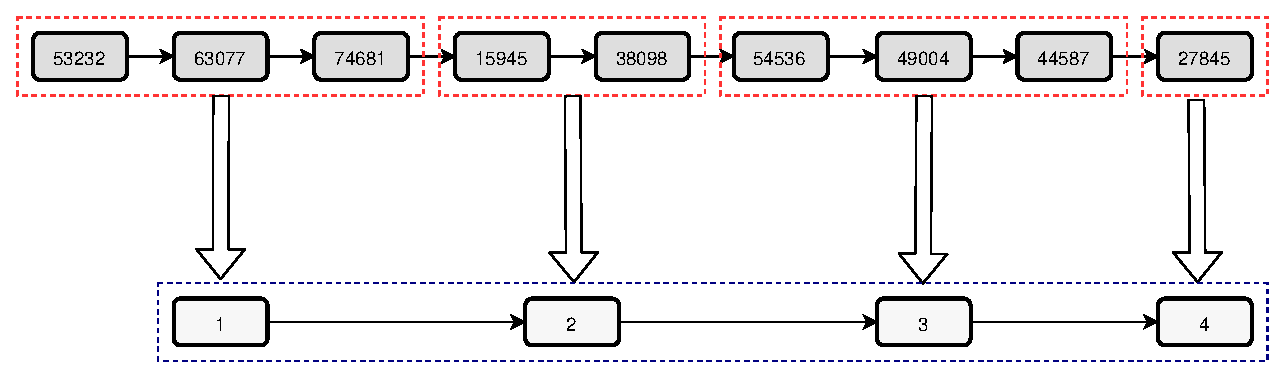
\includegraphics[width=1.0\textwidth]{Chapter2/Figs/Vector/Figure_cuantization.eps}
    \caption[Proceso de Cuantización]{Proceso de Cuantización.}
    \label{fig:Cuantization}
\end{figure}

En la literatura se ha encontrado que uno de los métodos más populares de análisis de conglomerados para la cuantización vectorial es el denominado k-means. Este método toma, en cuenta la distancia media entre los diferentes puntos para realizar el agrupamiento de los datos. Sin embargo, la condición de los datos que se están modelando en este trabajo suponen una dificultad, pues los datos a agrupar son vectores binarios. Lo anterior implica que, usar una medida de distancia como la euclidiana probablemente no arroje buenos resultados, por lo que se propone en cambio usar la medida de distancia hamming. 

Dado que la técnica de k-means generalmente no se usa en conjunto con la distancia hamming, es interesante usar otro tipo de técnicas de agrupamiento. Por ejemplo, el método de k-moda es comúnmente usado para clasificar secuencias genéticas, teniendo en cuenta la distancia hamming. Este método tiene en cuenta la moda de las distancias entre los datos para realizar la tarea de agrupamiento.

En conclusión, dentro del proceso de cuantización vectorial de los datos se tuvieron en cuenta tres métodos. El método de K-means, el método de K-moda, y por último, un método que no hace uso de técnicas de clasificación, pero que le asigna un único identificador a cada observación. A partir de estos métodos, se puede contar con diferentes conjuntos de datos, los cuales sirven como insumo para realizar todo el proceso predictivo propuesto en este trabajo.

